\documentclass[tikz,border=10pt]{standalone}
\usepackage{amsmath}
\usepackage{amssymb}
\usepackage{tikz}
\usetikzlibrary{arrows.meta,calc}

\definecolor{figazul}{RGB}{2,132,199}
\definecolor{figrojo}{RGB}{220,38,38}
\definecolor{figverde}{RGB}{22,163,74}

\begin{document}
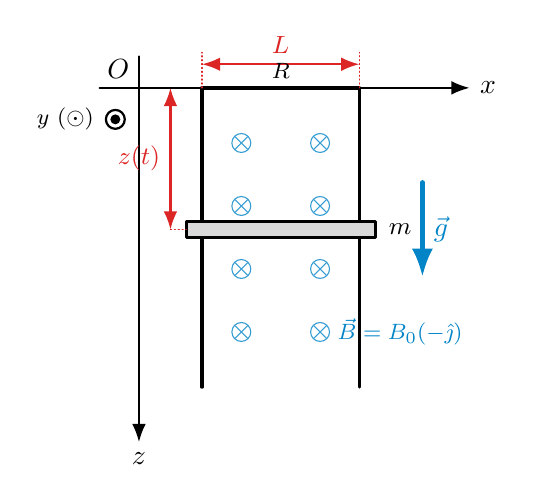
\begin{tikzpicture}[>=Latex, line cap=round, line join=round]
  % Ejes coordenados según convención del PDF:
  % x hacia la derecha, z hacia abajo
  \draw[->, thick] (-0.5, 0) -- (4.2, 0) node[right] {$x$};
  \draw[->, thick] (0, 0.4) -- (0, -4.5) node[below] {$z$};
  \node[above left] at (0,0) {$O$};

  % Eje y saliente (x \times y = z => y sale de la página)
  \draw[thick] (-0.3, -0.4) circle (0.12);
  \fill (-0.3, -0.4) circle (1.8pt);
  \node[left, font=\footnotesize] at (-0.45, -0.4) {$y$ ($\odot$)};

  % Circuito cerrado arriba (en z = 0 entre rieles)
  % Rieles en x = 0.8 y x = 2.8 (separación L = 2.0)
  \draw[very thick] (0.8, 0) -- (2.8, 0);

  % Rieles conductores verticales hacia abajo
  \draw[very thick] (0.8, 0) -- (0.8, -3.8);
  \draw[very thick] (2.8, 0) -- (2.8, -3.8);

  % Grilla de campo magnético uniforme B = B_0(-j_hat) (entrante \otimes)
  \foreach \gx in {1.3, 2.3} {
    \foreach \gz in {-0.7, -1.5, -2.3, -3.1} {
      \draw[thin, color=figazul!80] (\gx, \gz) circle (0.12);
      \draw[thin, color=figazul!80] (\gx-0.08, \gz-0.08) -- (\gx+0.08, \gz+0.08);
      \draw[thin, color=figazul!80] (\gx-0.08, \gz+0.08) -- (\gx+0.08, \gz-0.08);
    }
  }
  \node[right, font=\footnotesize, color=figazul] at (2.4, -3.1) {$\vec{B} = B_0(-\hat{\jmath})$};

  % Varilla conductora horizontal de masa m ubicada en z = -1.8
  \draw[very thick, fill=gray!30] (0.6, -1.9) rectangle (3.0, -1.7);
  \node[right, font=\small\bfseries] at (3.05, -1.8) {$m$};

  % Vector gravedad g hacia abajo
  \draw[->, ultra thick, color=figazul] (3.6, -1.2) -- (3.6, -2.4) node[midway, right, color=figazul] {$\vec{g}$};

  % Cota de separación L entre los rieles
  \draw[<->, thick, color=figrojo] (0.8, 0.3) -- (2.8, 0.3) node[midway, above, color=figrojo, font=\small] {$L$};
  \draw[densely dotted, thin, color=figrojo] (0.8, 0) -- (0.8, 0.45);
  \draw[densely dotted, thin, color=figrojo] (2.8, 0) -- (2.8, 0.45);

  % Cota de posición z(t) de la varilla
  \draw[<->, thick, color=figrojo] (0.4, 0) -- (0.4, -1.8) node[midway, left, color=figrojo, font=\small] {$z(t)$};
  \draw[densely dotted, thin, color=figrojo] (0.4, -1.8) -- (0.6, -1.8);

  % Resistencia R en la barra o en la barra superior
  \node[above, font=\footnotesize] at (1.8, 0) {$R$};

\end{tikzpicture}
\end{document}
